\documentclass[a4paper,12pt]{report}
\usepackage[T1]{fontenc}
\PassOptionsToPackage{defaults=hu-min}{magyar.ldf}
\usepackage[magyar]{babel}
\usepackage{graphicx}
\usepackage{url}

\title{HAI számítás nyílt forrású adatok alapján}
\author{Ozsváth Titusz}
\date{\today}

\begin{document}

\maketitle
\tableofcontents
\newpage

\chapter{Bevezetés}
\section{A feladat megfogalmazása}

\section{Felhasználási lehetőségei}

\section{Modellezés}

A modellezés három fontos és jól elkülöníthető szakaszból áll:

\begin{enumerate}
    \item Modellépítés
    \item Modell tesztelése
    \item Modell használata
\end{enumerate}

A szakdolgozat célja egy olyan modell létrehozása, amelyet a hétköznapokban is jól tudunk
használni, azaz a fenti felsorolás 3.\ pontja. A modellig azonban el kell jutni, amelyet az 1. és a
2.\ végrehajtásával tehetünk meg.

\chapter{A bementi adatok bemutatása}
Ebben a fejezetben kerülnek azok az adatok bemutatásra, amelyek alapján az első lépésben a modell
paraméterei meghatározásra kerülnek, illetve ha kész a modell ezen adatsorok új elemeivel
lehetséges megelőlegezett, de egyben meg is alapozott jóslatot tenni arra, hogy épp mekkora az
ország bruttó nemzeti összterméke.

Mivel a gazdaság az egyik legbonyolultabb rendszer a világon, így végtelen sok paraméteres
modelleket lehetne felállítani, amely a működését próbálja valamilyen formában megfogni. Ráadásul a
különböző szereplők, mint az utóbbi évtizedekben látjuk, sokszor irracionálisan viselkednek,
döntéseik sokszor kontextus függők, így egy teljes modellt felépíteni egy szakdolgozat keretében
lehetetlen vállalkozás.

A következő lehetőség, amely ebben a dolgozatban kihasználásra kerül, olyan fontos gazdasági
jellemzők összegyűjtése, amelyek bizonyítottan jól jósolják be a gazdaság egyes szektorainak vagy
egészének teljesítményét.

A projektfeladat keretében a következő jellemzőket választottam:

\begin{itemize}
    \item Energia:
          \begin{itemize}
              \item Üzemanyag fogyasztás (benzin és diesel)
              \item Üzemanyag árak (benzin és diesel)
              \item Gázárak
              \item Elektromos árak
          \end{itemize}
    \item Időjárás:
          \begin{itemize}
              \item Hőmérséklet
              \item Csapadék
              \item Levegő szennyezettség
          \end{itemize}
    \item Budapesti Értéktőzsde
    \item Gazdasági adatok
          \begin{itemize}
              \item Infláció
              \item Munkaerőpiac
          \end{itemize}
\end{itemize}

\section{Üzemanyag fogyasztás}

A mobilitás alapja még mindig a robbanómotoros közlekedési eszközök, így azok ára nagyon fontos
indikátora a gazdasági aktivitásnak. Minél alacsonyabb az ára az üzemanyagnak, annál több ember
teheti meg, hogy autózzon és annál több vállalkozásnak éri meg a termékeit szállítmányozni. És
természetesen minél alacsonyabb az üzemanyag ára, annál többet fogyasztanak belőle.

A magyarországi üzemanyag fogyasztást a Százhalombattán finomított üzemanyagok biztosítják messze a
legnagyobb százalékban. Százhalombattán továbbra is Barátság vezetéken szállított orosz uráli
típusú nyersolajat finomítanak még mindig, bár lassan folynak az átalakítási folyamatok, hogy más
forrásból tudjon fogadni nyers termékeket. Bár mindig megfigyelhető volt némi árkülönbség a brent
és az uráli típusú termékek között, az orosz-ukrán háború kiszélesedése után bevezetett szankciók
miatt a kereslet lecsökkent az uráli nyersolajra és így az ára nyomottá vált.

Ennek ellenére nincs különösebb kiskereskedelmi árkülönbség azon szomszédos országokkal összevetve,
ahol nem orosz termékeket dolgoznak fel. Így a nyereség legnagyobb részben a MOL-nál csapódik le.
Így elég, sőt indokolt a hazai árakkal dolgozni.

\begin{figure}[htbp]
    \centering
    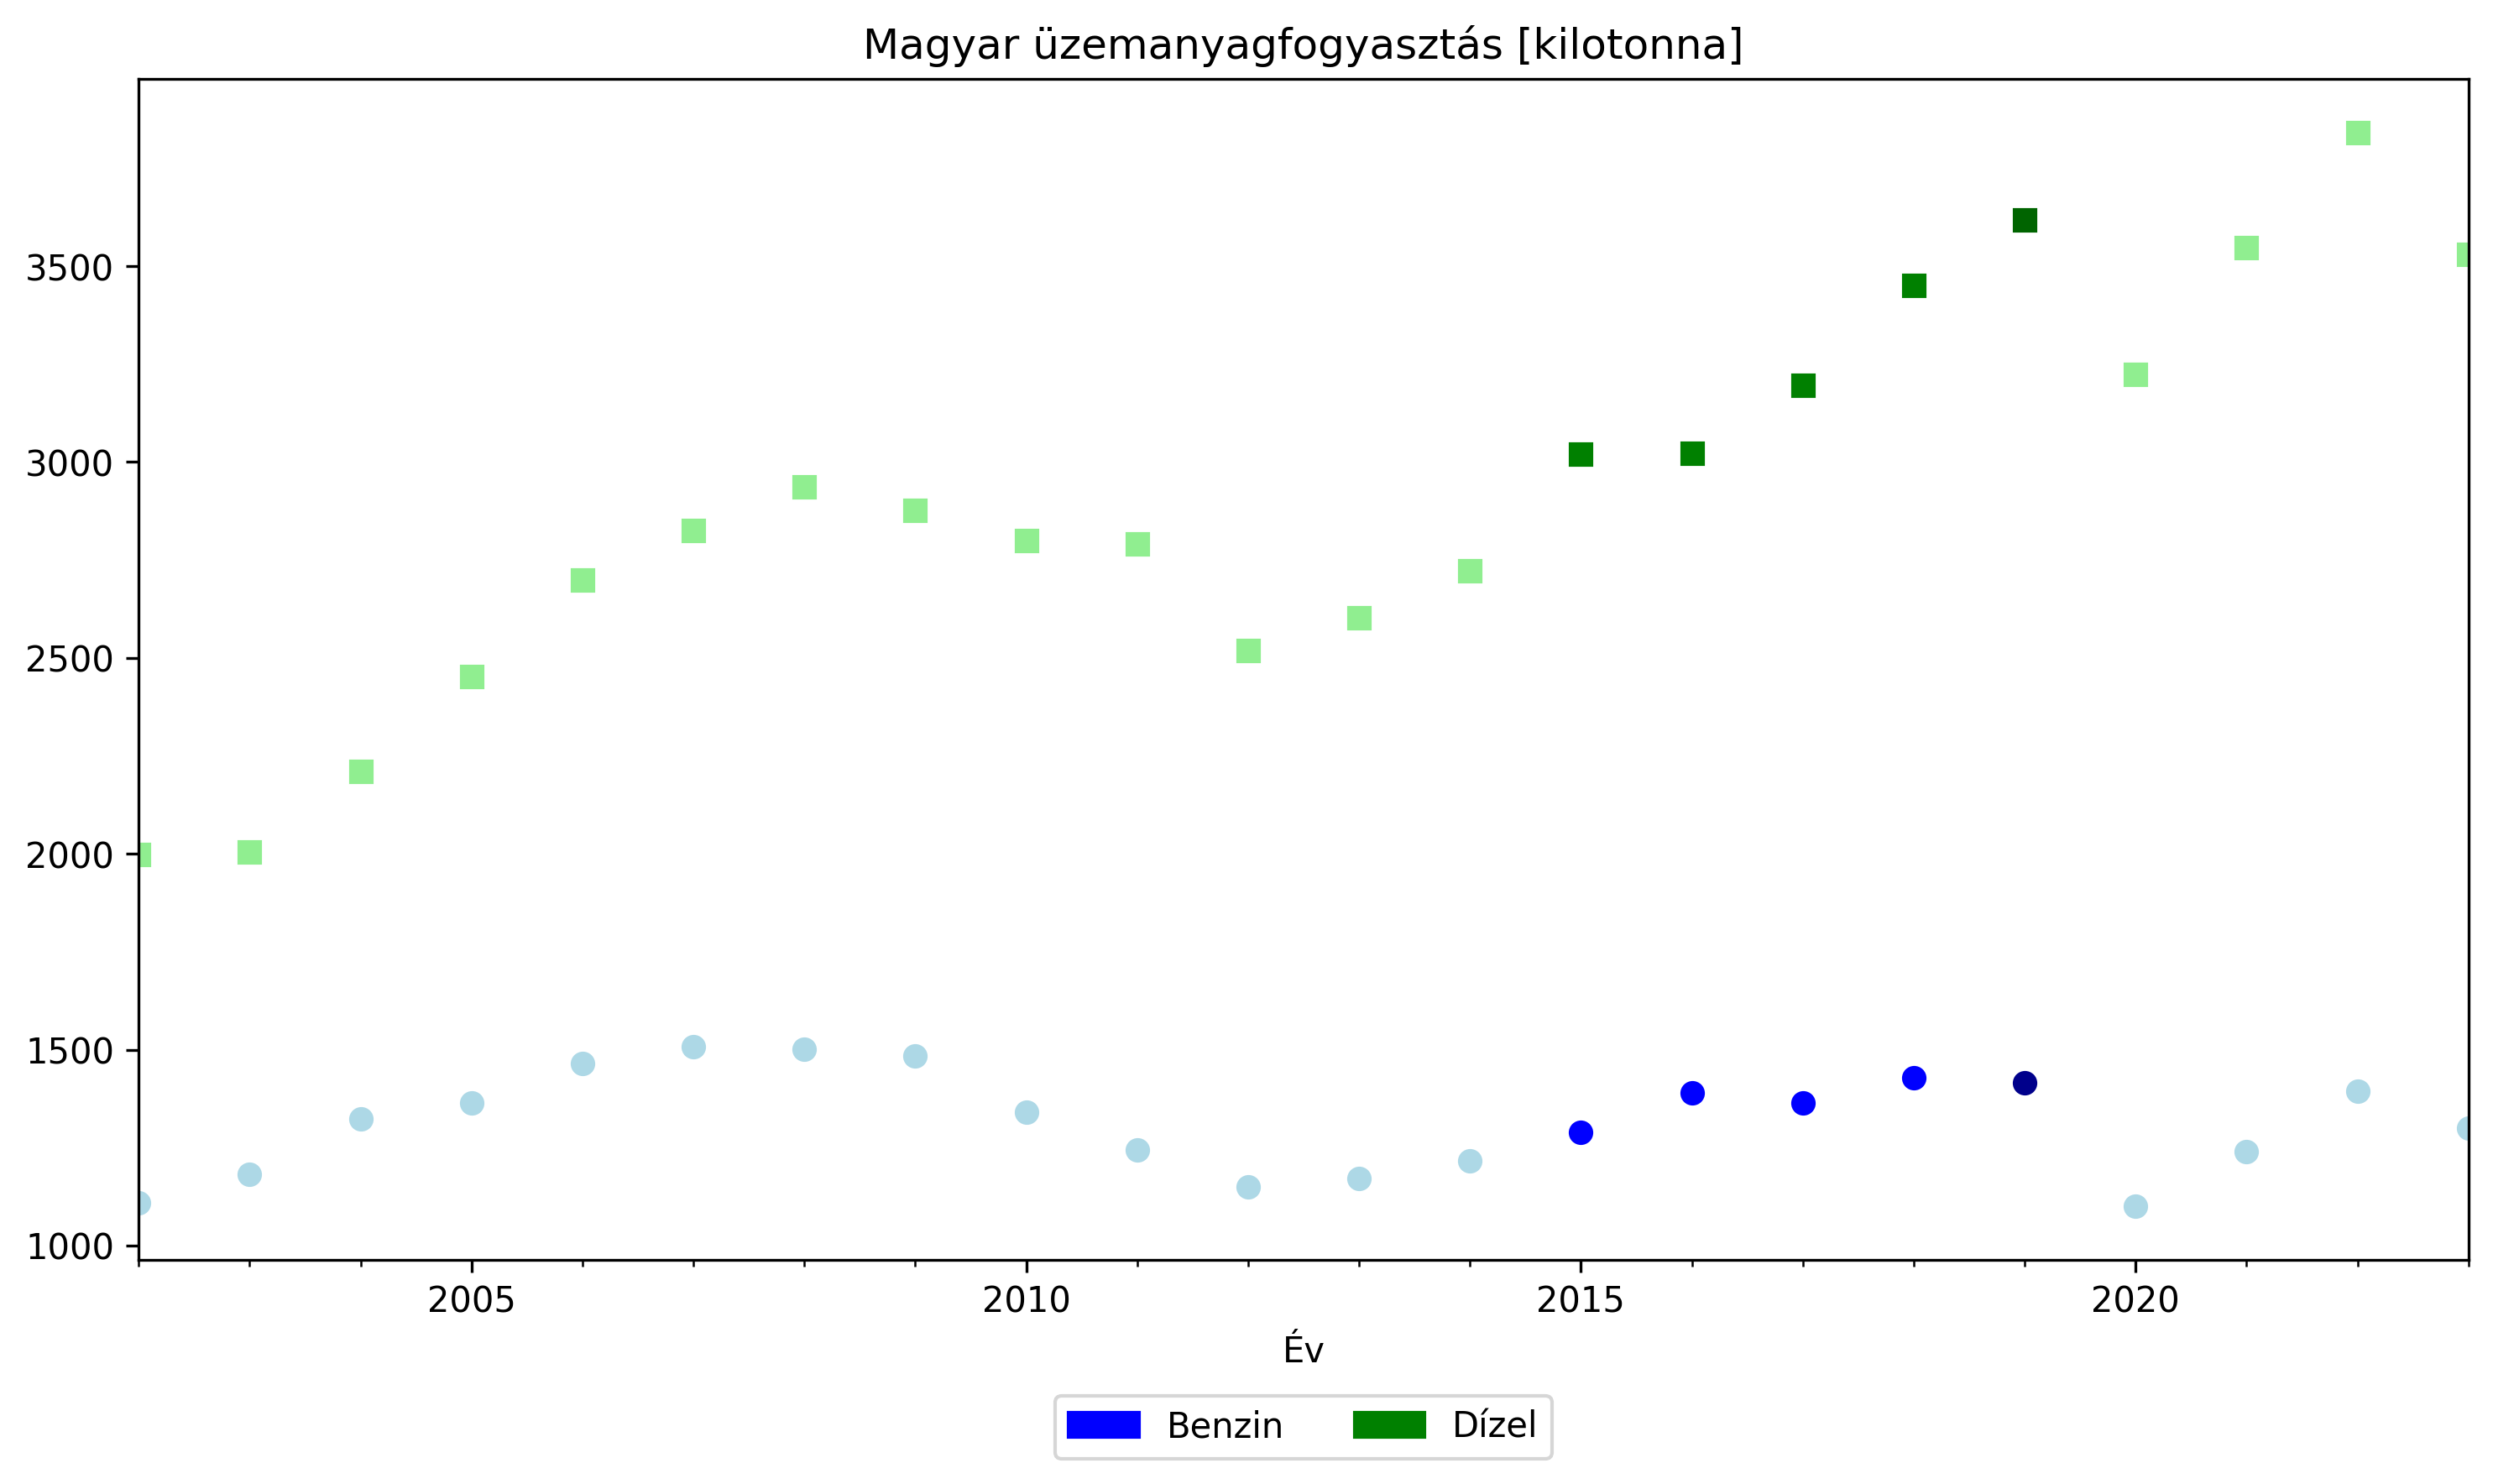
\includegraphics[width=1\textwidth, height=0.8\textheight, keepaspectratio]{../abrak/petrol_consumption.png}
    \caption{A magyar GDP alakulása szektorok szerint}\label{fig:petrol_consumption}
\end{figure}

Az ábrán zölddel a dízel, kékkel a benzin fogyasztás látható. Sötétebbel a projektfeladat keretében
vizsgált időszak (2015--2019) adatai lettek szedve. Megfigyelhetjük, a 2008-as válság miatti
fogyasztás visszaesés. Az erőteljes gazdasági növekedés 2014 körül tért vissza, utána viszont
meredeken emelkedett a fogyasztás. Olyan beruházások megvalósítása, mint a debreceni BMW gyár
építését megelőző tereprendezése, hónapokra 10--15\%-kal is meg tudták a dízel fogyasztást növelni.

A Covid lezárások visszavetették mindkét üzemanyag típus fogyasztását, de a benzin fogyasztásában
arányaiban jobban visszaesett, mert a benzint személygépkocsik használják nagyobb arányban és a
magánszemélyek mozgása sokáig korlátozva volt.

Ezzel szemben a 2022-ben bevezetett 480 forintos benzinársapka újból magasba emelte a fogyasztást,
sőt akkortájt még a benzinturizmus is megjelent a határaink mentén.

\section{Üzemanyag árak}

Az üzemanyag árak rugalmasabban alakulnak az üzemanyag fogyasztásánál, hiszen például megkezdett
beruházásokat nem hagynak félben amiatt, ha véletlenül kicsit drágább lesz a dízel.

Az előbb láthattuk tehát, hogy az üzemanyag kereslet rövidtávon rugalmatlan, addig a kínálatot
legalább két tényező befolyásolja még:
\begin{itemize}
    \item A különböző nemzetközi kartellszervezetek döntései.
    \item A piac várakozása, hiszen ha növekedés a konszenzusos várakozás, akkor megéri többet termelni,
          hiszen úgy is meg fogják venni. Így viszont túlkínálat is kialakulhat.
\end{itemize}

Épp utóbbira lehet példa a 2015--18-as időszak. A 2022-es választásra való felkészülést kísérő
kiköltekezés gyorsan megemelte az inflációt, majd az Ukrájnában kiújuló ellenségeskedés miatti aggodalom,
majd 2022 végén életbe lépő szankciók miatti csökkenő kereslet egekbe emelte az üzemanyag árakat. Ennek tartott ellent néhány hónapig a benzinársapka.

\begin{figure}[htbp]
    \centering
    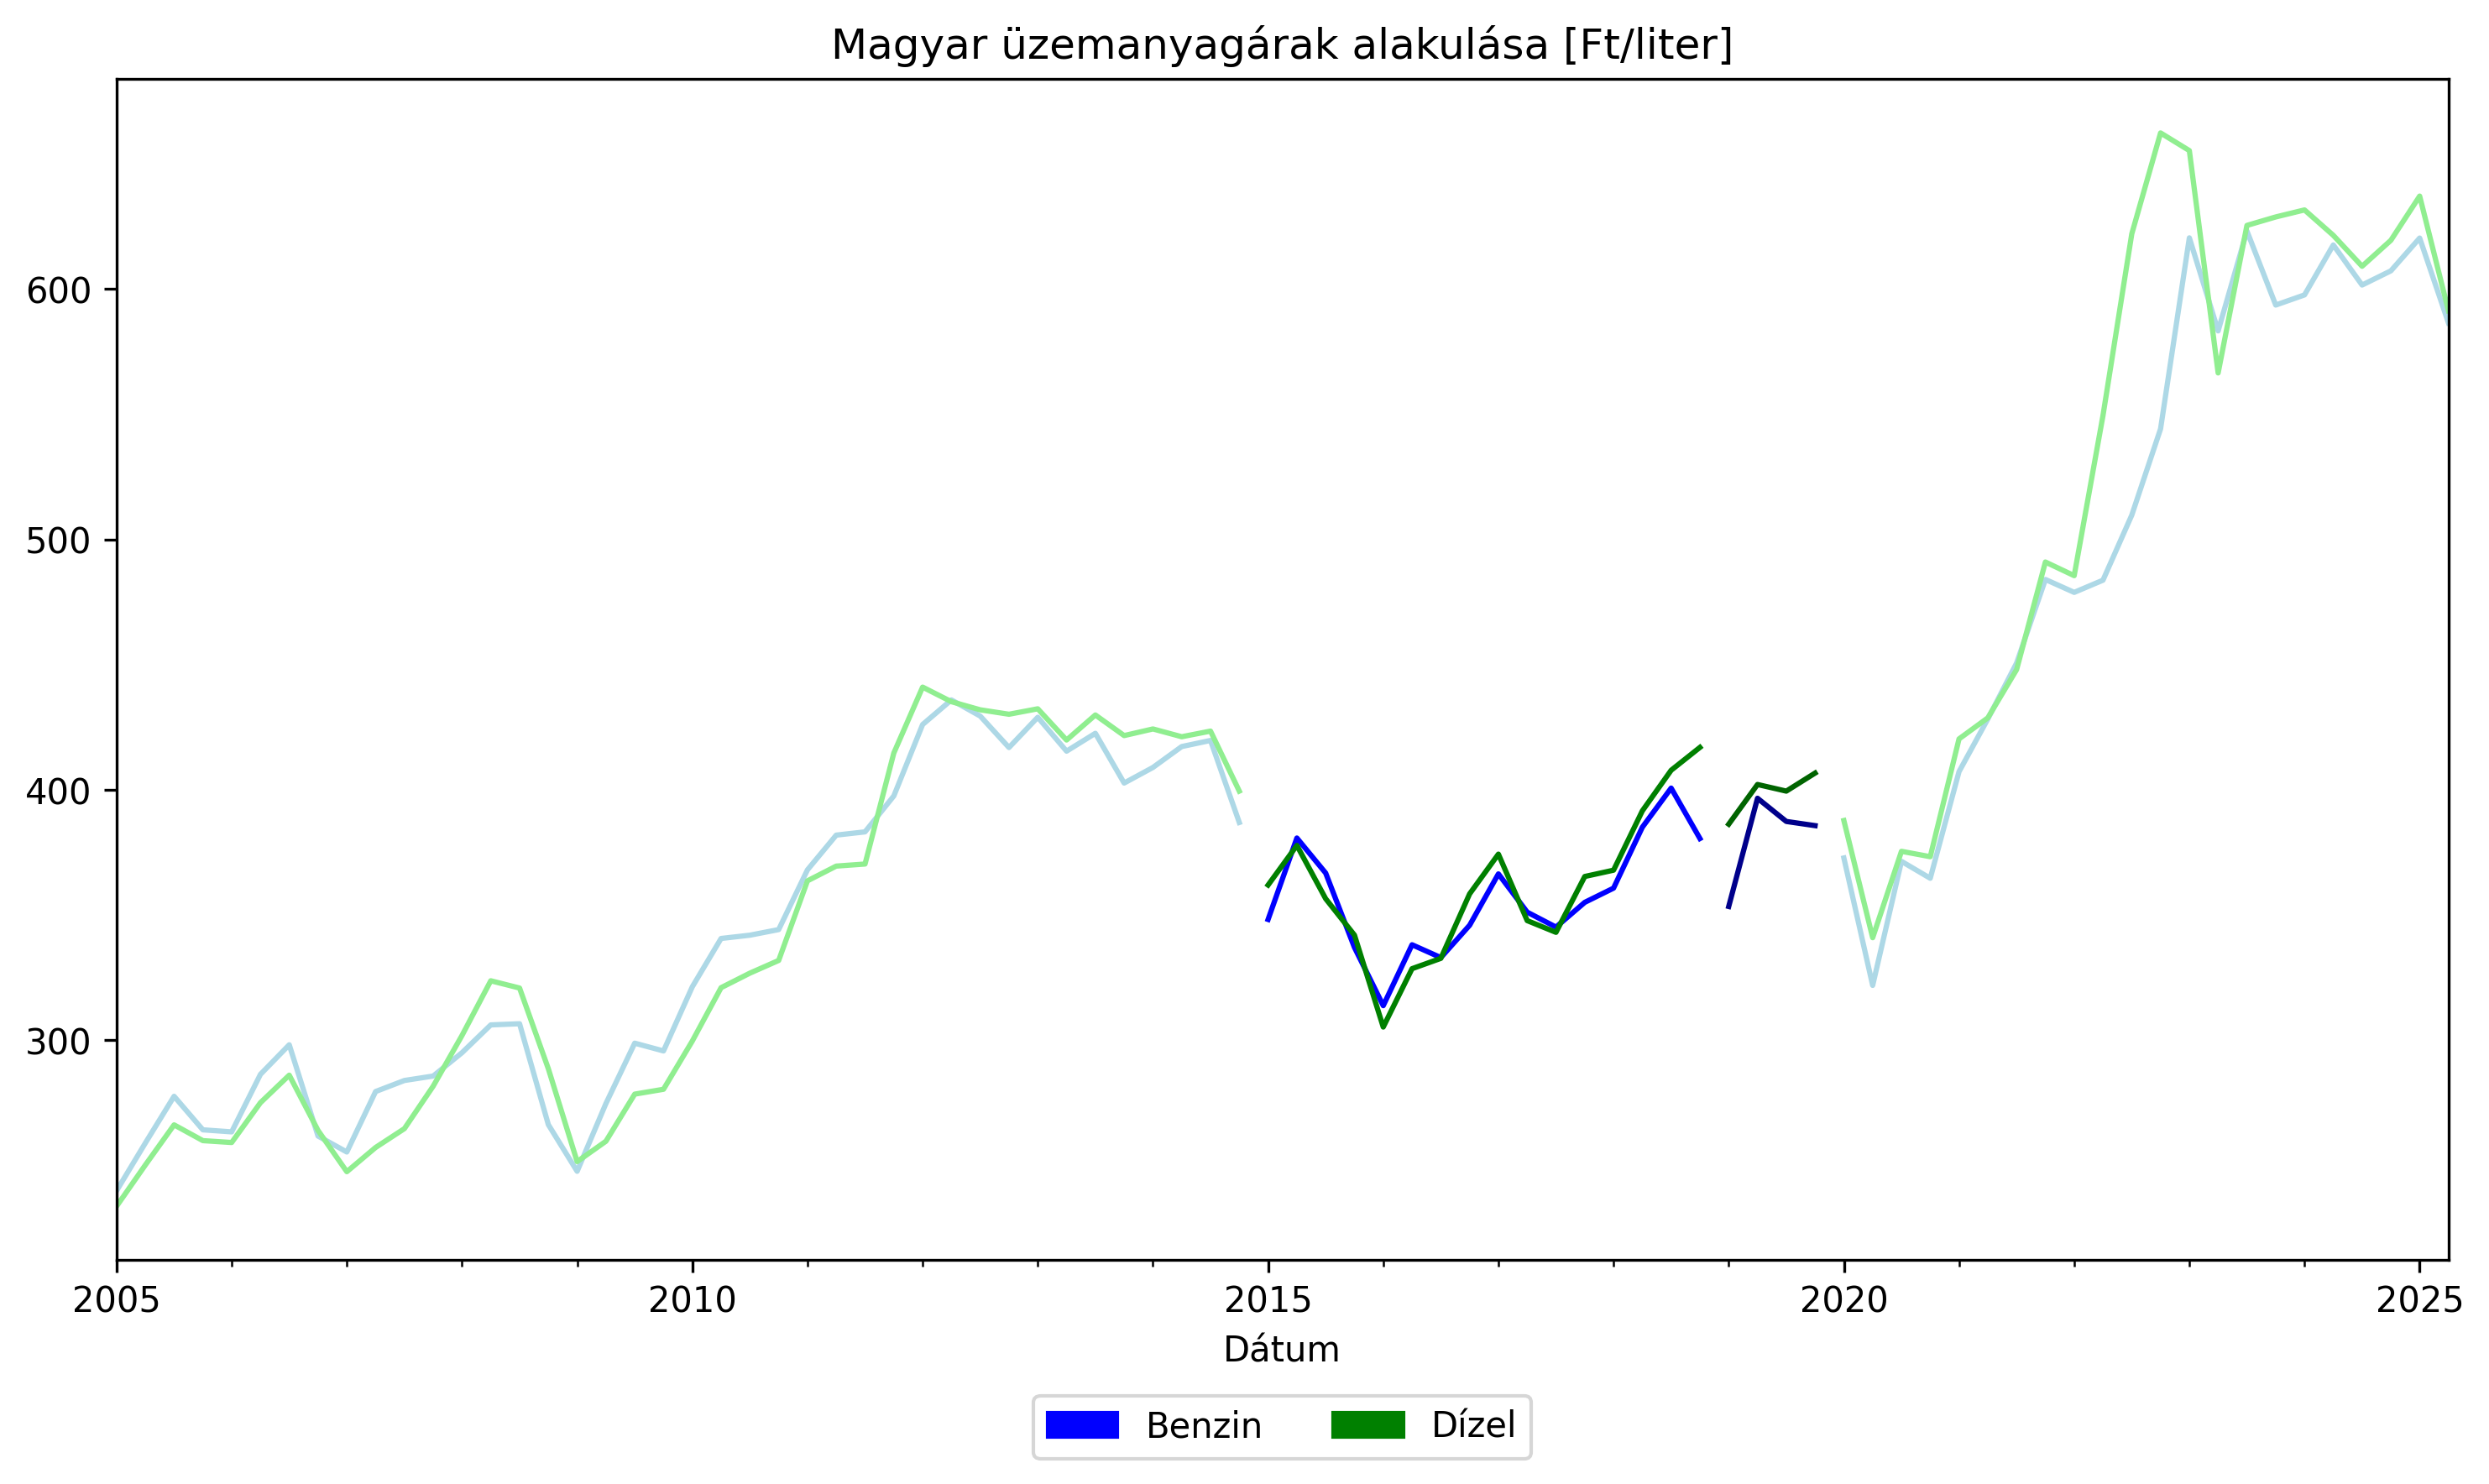
\includegraphics[width=1\textwidth, height=0.8\textheight, keepaspectratio]{../abrak/petrol_prices.png}
    \caption{A magyar GDP alakulása szektorok szerint}\label{fig:petrol_prices}
\end{figure}

\chapter{Modellek}
A kiírásban megfogalmazott feladat természetéből következik, hogy idősoros adatokat kell
feldolgozni, elemezni, az adatok alapján modellt építeni, az adatokat és végül magát a GDP-t
előrejelezni.

Idősoros adatokat több, alapvetően különböző megközelítésben lehet elemezni. A módszerek közötti
legalapvetőbb különbség az elemzés alapja:
\begin{itemize}
    \item idő
    \item frekvencia
\end{itemize}

\section{Frekvenciavizsgálat alapja és lehetőségei}

Természetesen igaz az alapvető összefüggés:
\begin{equation}
    f = \frac{1}{T}
\end{equation}
ahol $f$ a frekvencia és $T$ a periódus. Azaz az idő és a frekvencia egymás reciprokai.

Fontos még megjegyezni, hogy T periódusidőnek állandónak kell lennie, így önmagában nem elég, ha
csak hétköznapokról van adatunk és a hétvégéről nincs. Pontosabban fogalmazva a
frekvenciatartománybeli vizsgálathoz még felül kell valamilyen módszerrel mintavételezni a mintát.

A frekvencia elemzés fontos sarokköve, hogy minden periodikus jel/minta felírható szinuszon
komponensek szuperpozíciójaként.

Továbbmenve a Nyquist-Shannon-féle mintavételezési tétel szerint az előzőekben említett Fourier
transzformáció legmagasabb frekvenciájú komponensének legalább kétszeresével kell mintavételezni,
ahhoz hogy a jel helyreállítható legyen. Erre egy példa lehet, hogy az emberi hallás 20 és 20 ezer
Hz között működik, így egy jó minőségű hangfelvételnek legalább 40 kHz-esnek kell lennie.

\subsection{A magyar elektromos áram fogyasztás frekvenciatartománybeli vizsgálata}

A MAVIR Zrt.\ honlapján teszi közzé a magyar villamosenergia mind az aktuális mind a historikus
fogyasztási adatokat különböző, akár 1 perces mintavételi idővel. Az adatok, amelyet itt ebben az
esettanulmányban bemutatok, az a 2015.\ január 1.\ éjféltől 2019.\ december 31.\ éjfélig terjedő
időintervallumban mért ``Bruttó hitelesített rendszerterhelése``. A vizsgálódásunknak az a célja,
hogy kimutassuk az elsőre nem feltétlenül látszódó ciklikusságokat.

\begin{figure}[htbp]
    \centering
    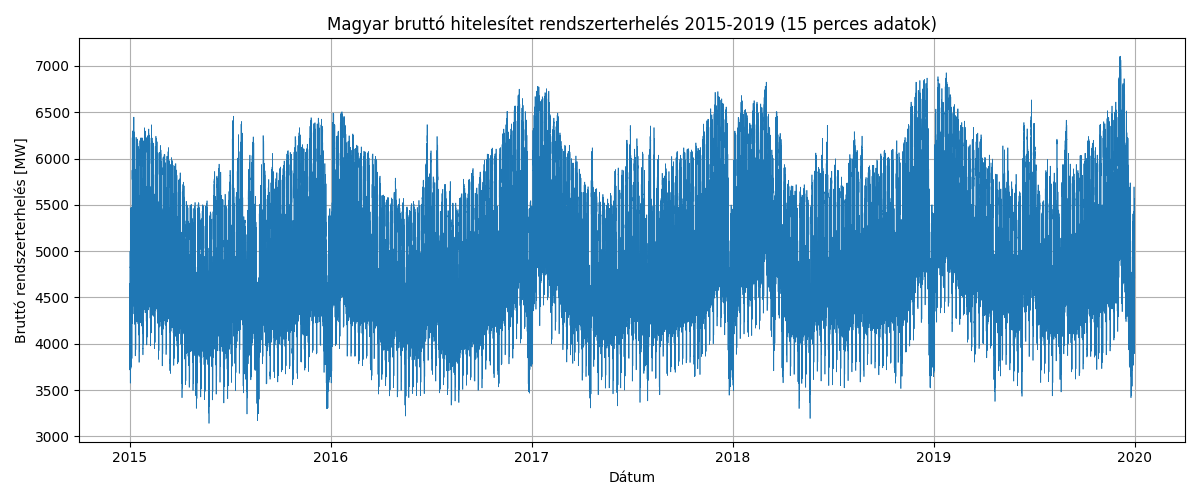
\includegraphics[width=1\textwidth, height=0.8\textheight, keepaspectratio]{../figures/electricity_time.png}
    \caption{Magyar bruttó hitelesítet rendszerterhelés 2015--2019 (15 perces adatok)}\label{fig:electricity_time}
\end{figure}

Előzetesen két periodicitás mindenképp logikusnak tűnik:
\begin{itemize}
    \item Éves periodicitás: a téli fűtési és a nyári légkondicionálási szokások ismétlődése.
    \item Napi periodicitás: a napi rutinok ismétlődése (világítás, fürdővíz).
\end{itemize}

Elvégezve a Fourier transzformációt és az eredményeket ábrázoljuk a következő diagrammot kapjuk:

\begin{figure}[htbp]
    \centering
    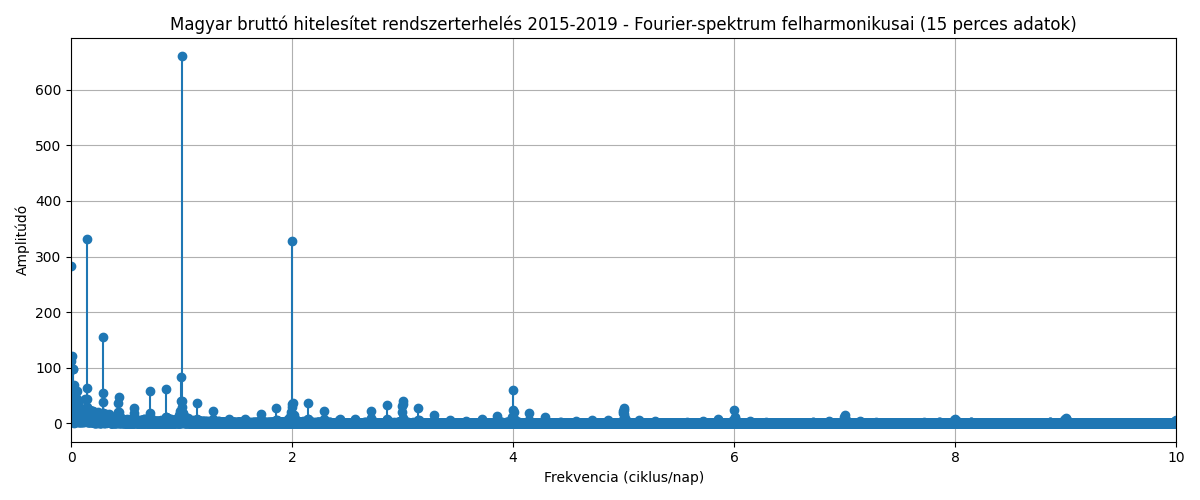
\includegraphics[width=1\textwidth, height=0.8\textheight, keepaspectratio]{../figures/electricity_fourier.png}
    \caption{Magyar bruttó hitelesítet rendszerterhelés 2015--2019 --- Fourier-spektrum felharmonikusai (15 perces adatok)}\label{fig:electricity_fourier}
\end{figure}

Leolvasva az öt legmagasabb értéket az ábráról, a következő frekvenciákat kapjuk:

\begin{itemize}
    \item 1 Hz (24 órás periódusidő): alapvető napi biológiai ritmus
    \item 2 Hz (12 órás periódusidő): reggeli és esti rutinok ismétlődése
    \item 0.142 Hz (168 órás periódusidő): heti ismétlődés a szokásokban (pl.\ hétvégi pihenés)
    \item nullához közel (feltehetőleg 0.0274Hz): éves mintázatok
    \item 4 Hz (6 órás periódusidő): napon belüli leállások (étkezés, műszakváltás)
\end{itemize}

Két megjegyzés:

\begin{itemize}
    \item A konstans tagot az ábra nem tartalmazza.
    \item Az adatok aggregált fogyasztást, tehát a lakosság és az ipar együttes fogyasztását mutatja. Az
          ipari tevékenységek sok esetben aszinkron történnek a lakosságival, amelyre a szolgáltatók
          ösztönözni igyekeznek ügyfeleiket, például kedvezményes éjszakai díjszabással. Ez tompítja a napi
          ingadozásokat és kisebb amplitúdókat eredményez a frekvenciatartományban.
\end{itemize}

Az esettanulmányból is láthatjuk, hogy a frekvenciatartománybeli vizsgálatok rámutathatnak fontos
tudásra a mintával kapcsolatban, ezek közöl is a legfontosabb a periodicitás. Ha ezt a GDP-re
vonatkoztatjuk, akkor rejtett üzleti ciklusokat feldezhetünk fel vele. Akár nagyon rövid, akár sok
éves ciklusokat.

Azonban a frekvenciatartománybeli vizsgálat több egyéb kérdést is felvet, amelyekből kettőt itt
megemlítek:

\begin{itemize}
    \item hiányzó adatok az adatsorban
    \item nehezen kezelhetők a gazdasági és politikai válságok hatásai
\end{itemize}

\chapter{A kimeneti adatok bemutatása}
\input{fejezetek/04_kimeneti_adatok.tex}

\chapter{Eredmények bemutatása és értelmezése}
\input{fejezetek/05_eredmenyek_bemutatasa.tex}

\chapter{Következő lépések}
További adatforrások bevonása:
\begin{itemize}
    \item Budapest Airport repülési adatai
    \item profession.hu
\end{itemize}
\end{document}
